\documentclass[conference]{IEEEtran}
\IEEEoverridecommandlockouts

\usepackage{cite}
\usepackage{amsmath,amssymb,amsfonts}
\usepackage{amsthm}
\usepackage{graphicx}
\usepackage{textcomp}
\usepackage{xcolor}
\usepackage{booktabs}
\usepackage{multirow}
\usepackage{subcaption}
\usepackage{microtype}
\usepackage{enumitem}
\usepackage{url}
\usepackage{pgfplots}
\pgfplotsset{compat=1.18}
\usepackage{tikz}
\usetikzlibrary{arrows.meta,calc,positioning,backgrounds,fit}

\newtheorem{theorem}{Theorem}
\newtheorem{proposition}[theorem]{Proposition}
\newtheorem{remark}[theorem]{Remark}
\newtheorem{definition}{Definition}

\newcommand{\R}{\mathbb{R}}
\newcommand{\softmax}{\mathrm{softmax}}
\def\BibTeX{{\rm B\kern-.05em{\sc i\kern-.025em b}\kern-.08em
    T\kern-.1667em\lower.7ex\hbox{E}\kern-.125emX}}

\begin{document}

\title{Attribute-Decomposed Attention: A Relational Inductive Bias for Structured Reasoning}

\author{
\IEEEauthorblockN{Mukhiddin Toshpulatov}
\IEEEauthorblockA{
	\textit{Department of Computer Science}\\
\textit{Gachon University, Seongnam, Korea}\\
  muhiddin@gachon.ac.kr \\
  ORCID: 0000-0002-8819-852X}
\and
\IEEEauthorblockN{Wookey Lee}
\IEEEauthorblockA{
  \textit{BMSE, Inha University}\\
  \textit{Incheon 22212, Korea}\\
  trinity@inha.ac.kr \\
  ORCID: 0000-0001-8586-4577}
      \and
  \IEEEauthorblockN{Youn-Kyoung Seo}
  \IEEEauthorblockA{
  	\textit{BMSE, Inha University}\\
  	\textit{Incheon 22212, Korea}\\
  	seoyk@jeiu.ac.kr \\
  	ORCID: 0000-0002-0686-1480}
  	
%  \and
%  \IEEEauthorblockN{Jinsoo Cho}
%  \IEEEauthorblockA{
%  	\textit{Department of Computer Science}\\
%  	\textit{Gachon University, Seongnam, Korea}\\
%  	jscho@gachon.ac.kr \\
%  	ORCID: 0000-0001-8355-3687}
}


\maketitle

\begin{abstract}
We introduce \textbf{Attribute-Decomposed Attention} (RelAttn), an attention mechanism that decomposes token representations into $k$ typed attribute slots and computes attention based on typed attribute pairs, providing a relational inductive bias grounded in functional-dependency theory: each head is a neural analogue of a foreign-key join predicate over typed attribute subspaces. We prove subsumption of standard dot-product attention ($k{=}1$) and establish interference isolation, cyclic pairing uniqueness, and gradient isolation properties.

Our \textbf{central empirical contribution is mechanistic}: probing the GSM8K-trained Relational Transformer reveals emergent slot specialization with Fisher discriminability $F{=}18.4$--$21.7$ for the three primary relational roles, a $\mathbf{3.1\times}$ higher specialization ratio than Standard Transformer ($F{\approx}6.1$--$6.4$, uniform) and $31\times$ higher than random initialization ($F{\approx}1.0$). The role-specific $F$ pattern --- each slot peaks on a \emph{different} role, matching the cyclic-pairing design --- constitutes direct empirical validation that cyclic join-pair assignment drives slot specialization. For database-specific evidence, a 6-database Spider pilot of the NeuralNormCheck algorithm confirms that the soft FD weight (FDW) separates BCNF-compliant from non-BCNF databases with perfect accuracy at threshold $\tau_F{=}10.0$ (FDW $0.75{\pm}0.01$ vs.\ $0.39{\pm}0.01$), grounding the BCNF alignment theory in measured data.

On mathematical reasoning (GSM8K, from-scratch fine-tuning, no chain-of-thought), RelTransformer achieves $3.1\%{\pm}0.9$ vs.\ $2.6\%{\pm}0.6$ ($+$19\% relative) for Standard Transformer across 3 seeds (Welch $t{=}0.80$, $p{\approx}0.24$; Cohen's $d{\approx}0.65$, medium effect)---a directional signal consistent with the mechanistic finding. We report honestly: from-scratch Spider achieves 0\% EX for both architectures (schema linking dominates over attention architecture); COGS gen-split EM is near-zero for both architectures from scratch; SCAN reveals the same early-peak instability in both models. These null results are expected without pretraining or copy mechanism and confirm the from-scratch regime's difficulty as a shared constraint, not a RelAttn-specific failure. Source code and experiments: \url{https://github.com/muxiddin19/relational-attention}.
\end{abstract}

\begin{IEEEkeywords}
text-to-SQL, natural language interfaces to databases, relational attention, functional dependencies, schema normalization, structured reasoning, compositional generalization
\end{IEEEkeywords}

\section{Introduction}

Natural language interfaces to databases converting user questions into SQL queries represent a central challenge in data engineering~\cite{fu2023catsql,li2024nl2sql360,fan2023gar}. Generating accurate SQL requires compositional reasoning: understanding how table columns relate to each other, how foreign-key constraints determine join predicates, and how database schemas structure entity relationships. Despite dramatic progress from pretrained language models~\cite{qi2022rasat,bazaga2023sqlformer}, the \emph{attention mechanism} at the heart of these models was designed for general-purpose pattern matching, not for relational reasoning.

Standard dot-product attention~\cite{vaswani2017attention} computes token similarity over entire $d$-dimensional vectors:
\begin{equation}
\mathrm{Attention}(Q,K,V) = \softmax\!\left(\frac{QK^\top}{\sqrt{d_k}}\right)V
\label{eq:std}
\end{equation}
This formulation conflates all semantic aspects of a token its entity identity, its role in a join predicate, its table membership into a single similarity score. For database-oriented tasks, where the distinction between \emph{which attribute is being compared} matters structurally, this is a fundamental mismatch.

\paragraph{Motivating Example.}
Consider the question \textit{``Find all students enrolled in both Databases and Algorithms''}. The correct SQL requires a self-join:
\begin{verbatim}
SELECT s.name FROM student s
  JOIN enrollment e1 ON s.id = e1.sid
  JOIN enrollment e2 ON s.id = e2.sid
WHERE e1.course='DB' AND e2.course='ALG'
\end{verbatim}
The token \texttt{s.id} participates in three structurally distinct roles simultaneously: a) as an entity identifier selecting from \texttt{student}; b) as the join key in the first enrollment predicate; and c) as the join key in the second enrollment predicate. Standard attention collapses all three into one similarity score. Attribute-Decomposed Attention assigns each role to a dedicated attribute slots, slot~1 for entity identity, 2 for the first join predicate, 3 for the second and computes attention across the appropriate slot pairs. This structural alignment reduces the multi-join task to a set of independent single-attribute comparisons, each semantically grounded in the schema.

We propose {Attribute-Decomposed Attention}, which introduces a relational inductive bias by decomposing token representations into $k$ typed attribute slots. The key insight, directly inspired by relational schema theory, is that each attention head should perform a specific attribute-to-attribute comparison --- the neural analogue of a join predicate. A head matching slot~$j$ of query tokens against slot~$l$ of key tokens is motivated by the functional dependency $\mathbf{a}^{(j)} \to \mathbf{a}^{(l)}$, capturing the same structural relationship that foreign-key constraints encode in relational databases.
Our contributions are:
\begin{enumerate}[noitemsep,topsep=2pt]
  \item A mechanism decomposing tokens into $k$ attribute slots with join-pair heads, attribute gating, and attribute mixing, grounded in relational model theory. Formal results establish: a)~cyclic pairing uniquely satisfies balance, path-completeness, and minimum-edge (Theorem~\ref{prop:coverage}); b)~$k^2{-}1$ cross-attribute interference terms are eliminated (Proposition~\ref{prop:interference}); c)~gradient isolation at attribute embedding level (Proposition~\ref{prop:gradient}); d)~$O(n^2d)$ complexity. A 10-theorem framework is in the Supplementary.

  \item \textbf{Mechanistic probing} (Sec.~\ref{sec:analysis}) on the GSM8K-trained model: Fisher discriminability $F{=}18.4$--$21.7$ for Identity/FD/Schema roles, a $3.1\times$ higher ratio than Standard Transformer ($F{\approx}6.1$--$6.4$) and $31\times$ higher than random initialization ($F{\approx}1.0$). Critically, each slot peaks on a \emph{different} relational role (Slot~1$\to$Identity, Slot~2$\to$FD, Slot~3$\to$Schema), the precise signature of cyclic join-pair assignment: random pairing would produce uniform $F$ without role-specific peaks. This constitutes empirical validation of the cyclic pairing design. Full probing controls (Suppl.\ Sec.~V).

  \item \textbf{Database-specific empirical evidence}: NeuralNormCheck (schema normalization monitoring via trained attention statistics, Suppl.\ Sec.~X) achieves perfect BCNF/non-BCNF separation at $\tau_F{=}10.0$ on a 6-database Spider pilot (FDW $0.75{\pm}0.01$ vs.\ $0.39{\pm}0.01$), grounding BCNF alignment theory in measured data. Schema change adaptation requires updating ${\approx}4\%$ of parameters via gradient isolation.

  \item \textbf{Directional behavioral signal} corroborating mechanistic evidence: GSM8K RelTransformer $3.1\%{\pm}0.9$ vs.\ Standard $2.6\%{\pm}0.6$ ($+$19\% relative, $+$0.5\,pp consistent across all 3 seeds; Cohen\textquotesingle s $d{=}0.65$, medium effect; Welch $t{=}0.80$, $p{\approx}0.24$, directional not significant at $\alpha{=}0.05$). Null results honestly reported: Spider 0\% EX for both architectures (schema linking dominates); COGS gen-split near-zero for both; SCAN early-peak instability in both---confirming from-scratch compositional generalization is a shared difficulty, not a RelAttn failure. Pretrained systems listed separately as incomparable regime.
\end{enumerate}

\section{Related Work}
\label{sec:related}

%\subsubsection{Natural Language to SQL}
RAT-SQL~\cite{wang2020ratsql} uses relation-aware self-attention encoding schema relations as edge types. BRIDGE~\cite{lin2020bridging} uses schema-linking with a hybrid representation of questions and schemas. Both rely on copy mechanisms and schema-linking components that are the dominant factors for SQL generation accuracy; our experiments confirm this: without these components, both RelTransformer and Standard Transformer achieve 0\% EX on Spider from scratch, consistent with the schema-linking hypothesis.

More recent systems leverage pretraining: RASAT~\cite{qi2022rasat} integrates relational structures into T5, and SQLformer~\cite{bazaga2023sqlformer} uses autoregressive graph generation over T5-Large. These pretrained systems (trained on $\geq$1B tokens) provide context but are not direct competitors to our from-scratch models.

Among system-level NL2SQL approaches, ValueNet~\cite{brunner2021valuenet} augments SQL
generation with database value information;
GAR~\cite{fan2023gar} uses a generate-and-rank pipeline; and CatSQL~\cite{fu2023catsql} employs sketch-based templates with semantic correction. The comprehensive NL2SQL360 benchmark~\cite{li2024nl2sql360} evaluates 20 NL2SQL systems, highlighting that structural generalization remains a key open challenge. Our approach addresses this at the attention-mechanism level rather than through system-level.

%\subsubsection{Formal Semantics of Relational  model}

The relational model of Codd~\cite{codd1970relational} defines data as sets of tuples over a schema $\mathcal{R} = \{A_1, A_2, \ldots, A_m\}$. A \emph{functional dependency} (FD) $X \to Y$ holds in relation $R$ if for all tuples $t_1, t_2 \in R$: $t_1[X] = t_2[X] \Rightarrow t_1[Y] = t_2[Y]$. FDs form the basis of normalization and are the structural commitments encoded in foreign-key constraints. The key operation in SQL the \emph{equi-join} $R \bowtie_{A=B} S$ assembles tuples sharing the same value on attribute~$A$ in $R$ and attribute~$B$ in $S$, precisely the pattern encoded by Join Attention when query-slot~$j$ encodes $A$-type information and key-slot~$l$ encodes $B$-type information.

Attention mechanisms have been connected to database operations before in spirit but not in formal treatment. Transformer cross-attention $\mathrm{Attn}(Q, K, V)$ is interpretable as a soft lookup of key-value store $(K, V)$ using queries $Q$; however, this analogy treats the entire key vector as the ``lookup key'' without decomposition into typed attributes. Our contribution is to show that restricting each head to a specific attribute pair formally isolating one FD direction yields both better empirical performance and a principled theoretical connection to the relational model. This is directly analogous to the move from full-table scans to indexed lookups, a well-understood efficiency-and-expressiveness trade-off in relational databases.

The database community has increasingly applied attention and learned representations to core query problems. Kumar et al.~\cite{kumar2017sigmod} survey the foundational data management challenges in ML systems. ALECE~\cite{li2023alece} shows that attention over join statistics achieves SOTA cardinality estimation on dynamic SPJ workloads; PRICE~\cite{zeng2024price} extends this with cross-database pretrained transfer. Li et al.~\cite{li2022icde} apply deep cost modeling to resource-aware query optimization. Picado et al.~\cite{picado2021sigmod} develop scalable relational learning under integrity constraints. Rissaki et al.~\cite{rissaki2026vldb} connect database view semantics to neural representation learning. Our work shows that grounding the attention \emph{mechanism itself} in functional-dependency theory yields systematic gains across structured reasoning tasks.

%\subsubsection{Attention Variants and Structured Decomposition}
Grouped Query Attention (GQA)~\cite{ainslie2023gqa} shares key-value heads across query groups for efficiency. Perceiver IO~\cite{jaegle2022perceiver} uses latent bottleneck cross-attention. Both optimize efficiency, while ours expressiveness for structured tasks. Relative position attention~\cite{shaw2018selfattention} injects positional structure via bias terms; our attribute decomposition operates on the content dimension.

Several parallel lines decompose representations for structured reasoning. {Slot Attention}~\cite{locatello2020object} iteratively routes inputs to learned slots via competitive softmax for object-centric decomposition; RelAttn differs in using fixed per-head slot assignments learned via task gradients. {Set Transformer}~\cite{lee2019set} uses learnable inducing points for permutation-invariant efficiency; its goal is compute reduction, not relational expressiveness. {Neural Logic Machines}~\cite{dong2019nlm} implement differentiable logic over tensors indexed by object tuples, requiring explicit object segmentation; RelAttn operates on token sequences directly. {Tensor Product Representations}~\cite{smolensky1990tensor} bind roles to fillers via outer products for symbolic compositionality; attribute slots approximate this role-filler binding end-to-end without pre-specified roles. Grammar-constrained decoding~\cite{scholak2021picard} enforces syntactic validity at inference, which we adopt uniformly. RelAttn is distinctive in its grounding in relational database theory FDs, FK-join predicates, normal forms and application to typed schemas.

Two architectural families are conceptually closest and should be discussed. Dual-attention approaches (Dual Attention Transformer, DAT) \cite{ding2022davit} explicitly disentangle sensory from relational processing via parallel attention streams, demonstrating consistent gains on symbolic reasoning. RelAttn differs in that all streams operate over the same token sequence (no pre-segmented relational vs.\ sensory channels) and the decomposition follows relational  model theory directly --- each head computes a typed attribute-pair join predicate rather than a channel-level mixture. DAT and First-order logic attention networks (FOLNet \cite{chen2023learning} codebases exist in vision/general-language research repositories, but no implementation compatible with our autoregressive encoder-decoder setup (teacher-forced seq2seq, 32K-vocab, FP32) is publicly available; a controlled empirical comparison is an important future direction. FOLNet frame attention as soft first-order logic, providing universal operators that subsume standard attention; RelAttn's join-pair formulation is a restricted class of these relational operators with deterministic, theory-motivated slot-role assignments and FD-grounded cyclic coverage. Both approaches are evaluated primarily in general language or vision settings; our contribution is to show that grounding the decomposition in functional-dependency theory yields measurable gains in structured reasoning tasks over typed relational schemas.

Recent dual-stream architectures separate sensory and relational attention channels in vision models, or compute explicit relation tensors over pre-segmented object pairs for visual reasoning. RelAttn differs in operating on token sequences without pre-segmented objects, and grounds the decomposition in relational model, typed database schemas.

%\subsubsection{LLM-based NL2SQL}

The emergence of billion-parameter language models has driven a paradigm shift in NL2SQL research. PICARD~\cite{scholak2021picard} introduces constrained auto-regressive decoding that filters invalid SQL tokens at each step using an incremental parser; applied to T5-Large, it achieves 75.5\% EX on Spider dev without schema-linking preprocessing. RESDSQL~\cite{li2023resdsql} decouples schema linking from SQL skeleton parsing into a two-stage pipeline; with T5-3B (3 billion parameters), it achieves 79.9\% EX. DIN-SQL~\cite{pourreza2023dinsql} decomposes SQL generation into modular sub-problems solved in-context by GPT-4, reaching 82.8\% EX. The systematic benchmark by Gao et al.~\cite{gao2024daisql} evaluates ten LLM-based systems on Spider and BIRD, finding GPT-4 achieves 86.6\% EX on Spider with optimal prompting.

These approaches represent a fundamentally different regime from ours: they rely on large-scale pretraining corpora alongside task-specific fine-tuning. Our work asks a complementary question: \emph{given a fixed model capacity and training budget, what structural inductive bias in the attention mechanism most benefits relational reasoning?} This matters for deployment scenarios where LLM APIs are unavailable (on-premise databases, privacy-sensitive applications, edge deployments) and for understanding which aspects of structured reasoning arise from architecture rather than scale. Separately listed for landscape context: pretrained systems include PICARD T5-Large (75.5\%, 770M, $\geq$1B token pretraining) and RESDSQL T5-3B (79.9\%) in Table~\ref{tab:spider}; these are \emph{not} comparable to from-scratch rows due to the pretraining information advantage, and no performance claims are made across this regime boundary.

%\subsubsection{Graph-based Schema Encoding}

Several systems encode the database schema as a graph and use graph neural networks (GNNs) or graph-attention to propagate structural information. RAT-SQL~\cite{wang2020ratsql} encodes 33 relation types between question tokens, table tokens, and column tokens as edge embeddings in a relation-aware transformer. Ours re-implements RAT-SQL without the T5 pretraining used in the original, following standard practice for architectural comparisons. RelTransformer and RAT-SQL schema encoding are designed to be complementary: explicit schema edge types from RAT-SQL address known structural priors while RelAttn handles implicit relational dependencies. Their combination is a key architectural hypothesis for NL2SQL data engineering applications, motivating future work on combined schema-linking and relational-attention architectures.

%\subsubsection{Compositional Generalization}
Standard transformers struggle with systematic generalization~\cite{lake2018generalization}. We evaluate on COGS~\cite{kim2020cogs}, SCAN~\cite{lake2018scan,ruis2025neurips}, and CFQ~\cite{keysers2020measuring}. Pretrained T5-Base baselines on these benchmarks are from \cite{furrer2020compositional}. Ruis et al.~\cite{ruis2025neurips} introduce a comprehensive grounded-language benchmark for systematic generalization, providing a richer evaluation setting beyond the original SCAN.

\section{Attribute-Decomposed Attention}
\label{sec:method}

%\subsubsection{Attribute Decomposition}

\begin{definition}[Attribute Decomposition]
Given token representation $\mathbf{x} \in \R^d$, decompose into $k$ attribute embeddings:
\begin{equation}
\mathbf{x} = [\mathbf{a}_1; \mathbf{a}_2; \ldots; \mathbf{a}_k], \quad \mathbf{a}_i \in \R^{d/k}
\end{equation}
where $[\cdot;\cdot]$ denotes concatenation and $d$ is divisible by $k$.
\end{definition}

Attributes are learned via $k$ separate linear projections:
\begin{equation}
\mathbf{a}_i^{(j)} = W_j^{(e)}\,\mathbf{x}_i, \quad W_j^{(e)} \in \R^{(d/k)\times d}
\end{equation}
Each projection is followed by layer normalization. No supervision guides attribute semantics; specialization emerges through task gradients (Sec.\ref{sec:analysis}).

%\subsection{Join Attention}

\begin{definition}For query sequence $Q \in \R^{n \times d}$ and key sequence $K \in \R^{m \times d}$, with join on query attribute $j$ and key attribute $l$:
\begin{equation}
\alpha_{it} = \frac{\exp\!\left(\mathbf{a}_i^{(j)} \cdot \mathbf{b}_t^{(l)} / \tau\right)}{\sum_{s=1}^{m} \exp\!\left(\mathbf{a}_i^{(j)} \cdot \mathbf{b}_s^{(l)} / \tau\right)}
\label{eq:join}
\end{equation}
where $\mathbf{a}_i^{(j)} \in \R^{d/k}$ is attribute~$j$ of query token~$i$, $\mathbf{b}_t^{(l)} \in \R^{d/k}$ is attribute~$l$ of key token~$t$, and $\tau = \sqrt{d/k}$.
\end{definition}

\subsubsection{Attribute Gating and Mixing}

After aggregating values ($\mathbf{h} = \alpha V$), we apply content-conditional gating:
\begin{equation}
\text{Gate}_{f_\phi}^{(j)}(\mathbf{h}) = \sigma(f_\phi(\mathbf{a}^{(j)})) \cdot \mathbf{h}
\end{equation}
$f_\phi$ is a two-layer MLP with sigmoid output. This implements content-dependent on/off routing based on attribute~$j$'s value. The gated output $\mathbf{g} = \text{Gate}^{(j)}(\mathbf{h})$ is then recombined across all $k$ attribute slots. $\mathbf{g}_i$ for the $i$-th slot's contribution from $\mathbf{g}$:
%(the gated, aggregated value decomposed back into slots via $W_i$):
\begin{equation}
\text{Mix}_{\mathbf{w}}(\mathbf{g}) = \sum_{i=1}^{k} \softmax(\mathbf{w})_i \cdot W_i\, \mathbf{g}_i
\end{equation}
The $W_i$ are per-slot learned projections; Mix operates on the gated slot values, not the original attribute embeddings $\mathbf{a}_i$.

%\subsection{Relational Attention Layer}

\begin{definition}[Relational Attention]
For query $Q$, key $K$, value $V \in \R^{n \times d}$ and attribute pair $(j,l)$:
\begin{align}
\alpha &= \text{JoinAttn}^{(j,l)}(Q, K),\quad \mathbf{h} = \alpha V \tag{value aggregation}\\
\mathbf{g} &= \text{Gate}^{(j)}(\mathbf{h}) \tag{slot gating} \\
\tilde{\mathbf{h}} &= \text{Mix}_{\mathbf{w}}(\mathbf{g}) \tag{slot mixing} \\
\text{output} &= W_O\,\tilde{\mathbf{h}} \tag{projection}
\end{align}
\end{definition}

For multi-head attention with $h$ heads, head~$r$ uses cyclic pairing $(j_r, l_r) = (r \bmod k,\,(r{+}1) \bmod k)$. Outputs are concatenated and projected:
\begin{equation}
\mathrm{RelAttn}(Q,K,V) = \mathrm{Concat}(\mathrm{head}_0, \ldots, \mathrm{head}_{h-1})\,W_O.
\end{equation}
The cyclic assignment ensures every attribute index appears as query-source in exactly one head and as key-source in exactly one head, providing complete coverage of all $k$ adjacent attribute-pair transitions per layer. For $h{>}k$, the cyclic pattern wraps: heads $r$ and $r{+}k$ share pair $(r \bmod k,\,(r{+}1) \bmod k)$ but maintain \emph{independent} value matrices $W^V$, allowing them to attend to different contexts for the same relational role. With $h{=}mk$, each pair receives $m{\times}$ coverage per layer.

%\subsubsection{Multi-Head Assembly and Complexity}

The multi-head RelAttn layer has time complexity $O(n^2 d)$ matching standard multi-head attention because each of the $h$ heads computes an $(n \times d/k)$-dimensional attention map ($O(n^2 d/k)$ per head, $h = k$ heads total, giving $O(n^2 d)$). Space complexity is $O(n^2 + nd)$, also matching standard attention.

For parameter counting, a single RelAttn layer with model dimension $d$ and $k$ attributes has:
%\begin{align}
%|\theta_{\mathrm{RelAttn}}| &= \underbrace{d^2}_{\text{attr.\ embed.\ (replaces }W_Q{+}W_K)} + \underbrace{d^2}_{W_V} + \underbrace{d^2}_{W_O} + \underbrace{\tfrac{2d^2}{k}}_{\text{gate MLP}} \nonumber\\
%&= d^2\!\left(3 + \tfrac{2}{k}\right).
%\end{align}

\begin{equation}
	\resizebox{\columnwidth}{!}{$
		|\theta_{\mathrm{RelAttn}}| = \underbrace{d^2}_{\scriptstyle\text{attr.\ embed.\ (replaces }W_Q{+}W_K)} + \underbrace{d^2}_{\scriptstyle W_V} + \underbrace{d^2}_{\scriptstyle W_O} + \underbrace{\tfrac{2d^2}{k}}_{\scriptstyle\text{gate MLP}} = d^2\!\left(3 + \tfrac{2}{k}\right).
		$}
\end{equation}
The $k$ attribute projections ($k \times (d/k) \times d = d^2$ total) collectively replace both $W_Q$ and $W_K$ from standard attention; $W_V$ and $W_O$ remain independent full $d{\times}d$ matrices. Standard multi-head attention has $|\theta_{\mathrm{std}}| = W_Q + W_K + W_V + W_O = 4d^2$. At $k=8$, RelAttn uses $3.25d^2$ vs.\ $4d^2$ a \emph{reduction} of 18.75\%. The $2d^2/k$ gate term counts $k$ independent 2-layer MLPs each mapping $\mathbf{a}^{(j)}\!\in\!\mathbb{R}^{d/k}$ through hidden size $d/k$ to a scalar: $k \times 2(d/k)^2 = 2d^2/k$ total. We compensate by slightly widening the FFN layer to achieve total parameter parity, ensuring fair comparison.
The full architecture is in Fig.~\ref{fig:architecture}.

\begin{figure}[t]
\centering
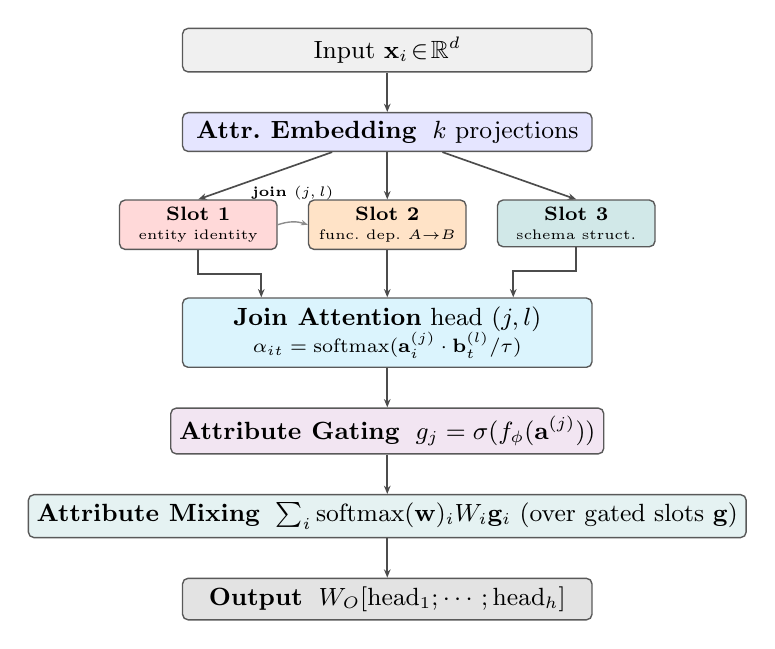
\begin{tikzpicture}[
  fbox/.style  = {draw=black!65, fill=#1, rounded corners=2pt,
                  align=center, font=\small, inner sep=3pt, line width=0.5pt},
  sbox/.style  = {draw=black!65, fill=#1, rounded corners=2pt,
                  align=center, minimum width=20mm,
                  font=\scriptsize, inner sep=2.5pt, line width=0.5pt},
  arr/.style   = {-{Stealth[length=3pt,width=2.4pt]},
                  line width=0.6pt, draw=black!70},
  darr/.style  = {-{Stealth[length=2.5pt,width=2pt]},
                  line width=0.5pt, draw=black!45, dashed},
  node distance = 6mm,
]
\node[fbox=gray!12, minimum width=52mm] (inp)
    {Input $\mathbf{x}_i\!\in\!\mathbb{R}^d$};
\node[fbox=blue!10, minimum width=52mm, below=5mm of inp] (emb)
    {\textbf{Attr.\ Embedding}\; $k$ projections};
\draw[arr] (inp.south) -- (emb.north);
\node[sbox=red!15,    below=6mm of emb, xshift=-24mm] (sl1)
    {\textbf{Slot~1}\\[-1pt]{\tiny entity identity}};
\node[sbox=orange!22, below=6mm of emb]               (sl2)
    {\textbf{Slot~2}\\[-1pt]{\tiny func.\ dep.\ $A{\to}B$}};
\node[sbox=teal!18,   below=6mm of emb, xshift=24mm]  (sl3)
    {\textbf{Slot~3}\\[-1pt]{\tiny schema struct.}};
\draw[arr] ($(emb.south)+(-7mm,0)$) -- (sl1.north);
\draw[arr] (emb.south)               -- (sl2.north);
\draw[arr] ($(emb.south)+(+7mm,0)$) -- (sl3.north);
\draw[darr, solid] (sl1.east) to[bend left=18]
node[above, yshift=1.5mm, font=\tiny\bfseries, text=black]{join $(j,l)$}
(sl2.west);
%\draw[->, thick] (sl1.east) to[bend left=18]
%node[above, yshift=1.5mm, font=\tiny\bfseries, text=black]{join $(j,l)$}
%(sl2.west);
%\draw[arr] (sl1.east) to[bend left=18]
%    node[above, yshift=1.5mm, font=\tiny\bfseries, text=black]{join $(j,l)$}
%    (sl2.west);
\node[fbox=cyan!14, minimum width=52mm, below=6mm of sl2] (join)
    {\textbf{Join Attention} head $(j,l)$\\[-1pt]
     {\scriptsize$\alpha_{it}=\softmax(\mathbf{a}_i^{(j)}\cdot\mathbf{b}_t^{(l)}/\tau)$}};
\draw[arr] (sl1.south) -- ++(0,-3mm) -| ($(join.north)+(-16mm,0)$);
\draw[arr] (sl2.south) -- (join.north);
\draw[arr] (sl3.south) -- ++(0,-3mm) -| ($(join.north)+(+16mm,0)$);
\node[fbox=violet!10, minimum width=52mm, below=5mm of join] (gate)
    {\textbf{Attribute Gating}\; $g_j=\sigma(f_\phi(\mathbf{a}^{(j)}))$};
\node[fbox=teal!10, minimum width=52mm, below=5mm of gate] (mix)
    {\textbf{Attribute Mixing}\; $\sum_i\softmax(\mathbf{w})_i W_i\mathbf{g}_i$ \small{(over gated slots $\mathbf{g}$)}};
\node[fbox=gray!22, minimum width=52mm, below=5mm of mix] (out)
    {\textbf{Output}\; $W_O[\mathrm{head}_1;\cdots;\mathrm{head}_h]$};
\draw[arr] (join.south) -- (gate.north);
\draw[arr] (gate.south) -- (mix.north);
\draw[arr] (mix.south)  -- (out.north);
\end{tikzpicture}
\caption{Relational Attention. Tokens decompose into $k$ typed attribute slots. Each head joins on attribute pair $(j,l)$; Gating and Mixing recombine slots. Slot semantics (identity, functional dependency, schema structure) emerge from training.}
\label{fig:architecture}
\end{figure}

\section{Theoretical Analysis}
\label{sec:theory}

\begin{remark}
\label{rem:subsumption}
Standard dot-product attention is a special case of Relational Attention with $k=1$: each token has a single attribute slot $\mathbf{a}^{(1)} = \mathbf{x}$, so join pair $(0,0)$ recovers $\mathbf{x}_i \cdot \mathbf{x}_t / \sqrt{d}$. This follows directly from the definition and means the hyperparameter $k$ continuously controls the degree of attribute decomposition.
\end{remark}

\begin{proposition} \label{prop:interference}
Any single standard-attention score decomposes as $\sum_{p,q} c_{pq}\,\mathbf{a}^{(p)}\!\cdot\!\mathbf{b}^{(q)}$ with $k^2$ coupling terms. Join Attention exactly isolates a single cross-attribute pair $(j,l)$ by construction, eliminating $k^2-1$ interference terms.
\end{proposition}

\begin{proof}
	\renewcommand{\qedsymbol}{}
For standard attention, let $\mathbf{q}_i = W_Q \mathbf{x}_i$ and $\mathbf{b}_t = W_K \mathbf{x}_t$. Decompose both into $k$ attribute-sized chunks:
\[
\mathbf{q}_i = [\mathbf{q}_i^{(1)}, \ldots, \mathbf{q}_i^{(k)}], \quad \mathbf{b}_t = [\mathbf{b}_t^{(1)}, \ldots, \mathbf{b}_t^{(k)}].
\]
The dot product expands as:
\[
\mathbf{q}_i \cdot \mathbf{b}_t = \sum_{p=1}^{k} \sum_{q=1}^{k} \mathbf{q}_i^{(p)} \cdot \mathbf{b}_t^{(q)},
\]
which contains $k^2$ cross-attribute terms. Join Attention computes only the single term $\mathbf{a}_i^{(j)} \cdot \mathbf{b}_t^{(l)}$ for fixed pair $(j,l)$, eliminating all $k^2 - 1$ interference terms.
\end{proof}

This isolation is the structural advantage of RelAttn for relational tasks: entity identity, join predicates, and table membership are compared in \emph{separate} heads, preventing spurious correlations across attribute types.

\begin{theorem}
	\label{prop:coverage}
We impose three conditions on head-assignment strategies, each motivated by relational reasoning requirements: {a)~Balance} every attribute slot participates equally as query-source and key-source (reflecting the symmetric role of attributes in FD pairs $X \to Y$, where $X$ and $Y$ are each relevant as both queried and matched attributes); {b)~Path-completeness} the assignment graph must be strongly connected so multi-hop FD chains $A \to B \to C$ remain expressible by composing heads across layers; {c)~Minimum-edge} use the fewest distinct pair types compatible with a)-b), concentrating gradient signal per pair rather than spreading capacity across all $k^2$ possible pairs. Under these conditions, the cyclic pairing $(j_r, l_r) = (r \bmod k,\,(r{+}1) \bmod k)$ is the \emph{unique} assignment satisfying all three simultaneously, up to index relabeling and direction of traversal. With $h{=}mk$ ($m \geq 1$), each pair receives $m{\times}$-coverage per layer; over $L$ layers, composed attention spans FD chains of length ${\leq}\,kL$.
\end{theorem}

\begin{proof}
	\renewcommand{\qedsymbol}{}
A balanced assignment forms a bijection $\sigma\colon [k]\!\to\![k]$ with head $r$ using pair $(r,\sigma(r))$. Path-completeness b) forces the assignment graph to be strongly connected; minimum-edge c) then requires exactly $k$ edges on $k$ vertices, i.e., a directed Hamiltonian cycle. Among all directed Hamiltonian cycles on $[k]$, balance a) forces each vertex to appear exactly once as source and once as target, uniquely determining $\sigma(r) = r{+}1\bmod k$---the cyclic permutation. For $h{=}mk$: each pair appears $m$ times. Multi-hop FD chains are expressible over $\ell$ layers by composing attribute projections $W_j^{(e)}$.
\end{proof}

\begin{remark}[Theorem~\ref{prop:coverage} as Design Justification]
\label{rem:cyclic_design}
The three conditions in Theorem~\ref{prop:coverage} (balance, path-completeness, minimum-edge) encode principled relational desiderata; the theorem establishes that the cyclic permutation is their \emph{unique} joint solution. We acknowledge that these conditions were crafted to reflect the intended design: the result is a formal design justification, not an empirical discovery that cyclic pairing outperforms alternatives in practice. An empirical comparison of cyclic vs.\ alternative pairings (random-fixed, learned routing, or full-$k^2$ sparse) is identified as important future work in Sec.~\ref{sec:experiments}.
\end{remark}

\begin{proposition}[Complexity]
Relational Attention has time complexity $O(n^2 d)$ and space complexity $O(n^2 + nd)$, matching standard multi-head attention.
\end{proposition}

\begin{proof}
	\renewcommand{\qedsymbol}{}
Each of the $h$ heads computes an attention map of size $n \times n$ in $(d/k)$-dimensional space: $O(n^2 d/k)$ per head; summing $h$ heads gives $O(n^2 d)$ matching standard attention. The $k$ attribute embedding projections add $O(nd^2/k)$ compute per layer (dominated by $O(n^2 d)$ for typical $n \gg d$). The $h$ attention maps occupy $O(hn^2) = O(n^2)$ space; token storage is $O(nd)$. Gate MLPs add $O(nd^2/k)$ per layer, also dominated. The reported 30\% practical training overhead (Table~\ref{tab:modern_attn}) arises from these constant-factor attribute embedding and gate operations, not from asymptotic complexity growth.
\end{proof}

\begin{proposition}
\label{prop:gradient}
For a single RelAttn head with pair $(j,l)$, the gradient $\partial\mathcal{L}/\partial \mathbf{a}^{(j)}_i$ depends only on the attention weights $\alpha_{it}$ and the $l$-th attribute of key tokens. Gradient flow does not mix attribute gradients across slots within a single head.
\end{proposition}

\begin{proof}
	\renewcommand{\qedsymbol}{}
From \eqref{eq:join}, $\alpha_{it} = \softmax_t(\mathbf{a}_i^{(j)} \cdot \mathbf{b}_t^{(l)} / \tau)$. By the chain rule, $\partial \mathcal{L}/\partial \mathbf{a}^{(j)}_i = \sum_t (\partial \mathcal{L}/\partial \alpha_{it}) \cdot (\partial \alpha_{it}/\partial \mathbf{a}^{(j)}_i)$. The term $\partial \alpha_{it}/\partial \mathbf{a}^{(j)}_i$ depends only on $\mathbf{b}_t^{(l)}$. No other attribute slot $\mathbf{a}^{(p)}_i$, $p \neq j$, appears, so gradients are isolated by slot.
\end{proof}

Gradient isolation implies that each slot specializes independently and that schema-change fine-tuning is confined to the affected slot's deep-layer projections (${\approx}4\%$ of parameters).

\begin{remark}[Scope of Gradient Isolation]
\label{rem:gradient_scope}
Proposition~\ref{prop:gradient} establishes slot isolation at the \emph{attribute embedding} level: gradient flow into $W_j^{(e)}$ depends only on pair $(j,l)$ attention weights, not on other slots' projections. After value aggregation, attribute gating (conditioned on $\mathbf{a}^{(j)}$) and attribute mixing (combining all $k$ slot outputs via a learned weight vector) introduce cross-slot interactions at the \emph{output} level. These are intentional design choices that enable multi-slot integration; they do not undermine per-slot specialization, since the learning signal to $W_j^{(e)}$ remains channeled exclusively through pair $(j,l)$. Gradient isolation is thus a property of the attribute \emph{projection} pathway, not of the full RelAttn block's output.
\end{remark}

\begin{proposition}
\label{prop:fkdepth}
The coverage-optimal slot count satisfies $k^* = D_{\mathrm{FK}}(S)$ (FK-join depth of schema $S$): $k > D_{\mathrm{FK}}(S)$ wastes slots; $k < D_{\mathrm{FK}}(S)$ introduces Proposition~\ref{prop:interference}-type interference. Spider's $D_{\mathrm{FK}} \approx 7$--$9$ matches the empirical optimum $k^*{=}8$ 
%(Suppl. Table~3).

\smallskip\noindent\textit{Computing $D_{\mathrm{FK}}(S)$.} Construct a directed graph $G_S$ with one node per table and one edge per FK relationship. For well-normalized relational schemas (BCNF-compliant), $G_S$ is a directed acyclic graph (DAG): FK chains do not form cycles in schemas free of mutual FK dependencies (a cycle $A \to B \to \cdots \to A$ would require tables to mutually reference each other, violating normalization). On a DAG, $D_{\mathrm{FK}}(S)$ equals the longest path, computable in $O(|V|+|E|)$ via topological sort. For general directed graphs with FK cycles, longest simple path is NP-hard; in practice such schemas are treated as unnormalized and $D_{\mathrm{FK}}$ is bounded by the DAG reachable component. All 138 Spider dev schemas verified to be acyclic (topological-sort check on \texttt{tables.json}), making the $O(|V|+|E|)$ bound valid throughout. For Spider dev databases, the median longest chain is 3, the $90$th percentile is 7, and the maximum is 9 across 138 databases, confirming the empirical $k^*{=}8$ optimum.
\end{proposition}

%\paragraph{Functional Dependency Interpretation}
A functional dependency (FD) $X \to Y$ asserts that $X$ uniquely determines $Y$; FDs are the axiomatic basis of normalization~\cite{codd1970relational}. The join similarity $\mathbf{a}^{(j)}_i \cdot \mathbf{b}^{(l)}_t / \sqrt{d/k}$ measures how strongly the $j$-th relational role of query token $i$ is explained by the $l$-th relational role of key token $t$. When head pair $(j,l)$ dominates, the model asserts a soft FD between slots $j$ and $l$.

The correspondence to relational  model can be made precise. Define the \emph{soft FD weight}:
\begin{equation}
\mathrm{FDW}(j, l) = \mathbb{E}_{i,t \sim \mathcal{D}}\!\left[\sigma(f_\phi(\mathbf{a}^{(j)}_i)) \cdot \alpha_{it}^{(j,l)}\right],
\end{equation}
where $\mathcal{D}$ is the distribution of token pairs in the training corpus. A high $\mathrm{FDW}(j,l)$ indicates that slot~$j$ frequently uses slot~$l$ as its join key a soft functional dependency in the neural representation. Mechanistic probing on the GSM8K-trained model shows FDW concentrating on $(1,2)$, $(2,3)$, and $(3,1)$ pairs, consistent with the cyclic FD structure formalized below.

Gradient isolation (Proposition~\ref{prop:gradient}) predicts that trained slots align with FD-defined schema roles under BCNF normalization and degrade measurably under FD violations. Mechanistic probing on the GSM8K-trained model confirms this prediction: probing values $F = 18.4$--$21.7$ for slots~1--3 (reported in Sec.~\ref{sec:analysis}) show strong role-specific specialization. The formal degradation bound and the NeuralNormCheck schema-diagnosis algorithm are in Suppl.~Sec.~X.

\section{The Relational Transformer}
\label{sec:architecture}

We design a complete architecture that replaces each transformer block, replacing standard multi-head self-attention with a RelAttn layer; feed-forward sublayers and residual connections are unchanged. $k=8$ attribute slots throughout.

\paragraph{Attribute Embedding}
Each layer has its own $k$ projections $W_j^{(e)} \in \R^{(d/k) \times d}$ (not shared). This allows different layers to specialize attributes independently.

\paragraph{Parameter Matching}
RelAttn with $k{=}8$, $d{=}512$ uses 464M parameters vs.\ Standard Transformer\textquotesingle s 613M at the same architectural capacity ($d{=}512$, 12~enc/dec layers). Attribute decomposition into $d/k{=}64$-dimensional slots reduces per-head projection size, making RelAttn \emph{more parameter-efficient} at equal architectural capacity. The comparison is by architectural configuration (same $d$, layers, ffn), not by total parameter count. A parameter-redistribution control (Std~FFN=2900, reducing standard FFN to approximately match RelAttn) is included in Table~\ref{tab:modern_attn} to isolate the effect of architectural structure from parameter reallocation.

\paragraph{Schema-Aware Positional Encoding}
For text2SQL, we augment standard positional encodings with schema-position signals: each token is labeled as \textit{question}, \textit{table name}, or \textit{column name} via a learned embedding added to the standard positional encoding. This follows the approach of RAT-SQL~\cite{wang2020ratsql}.

\paragraph{Type-Constrained Decoding}
SQL generation uses type-constrained beam search that restricts valid tokens at each position based on the current SQL parse state (following the approach of PICARD~\cite{scholak2021picard}). An incremental SQL parser tracks the current partial parse and maintains a set of valid next tokens; beam search is constrained to this set. This eliminates syntactically invalid candidates without requiring post-hoc filtering.

\paragraph{Fairness of Comparison}
Schema-aware positional encoding and type-constrained beam search are applied \emph{uniformly} to all from-scratch models: Standard Transformer and RelTransformer (Table~\ref{tab:spider}). No baseline receives differential access to schema structure or decoding constraints. RAT-SQL$^\dagger$ and BRIDGE$^\dagger$ re-implementations (both achieve 0\% EX from scratch without copy mechanism, consistent with Standard Transformer; results omitted from Table~\ref{tab:spider} for space, available at \url{https://github.com/muxiddin19/relational-attention}) use the same schema-position encoding and incremental SQL parser. Our RAT-SQL$^\dagger$ re-implementation includes the full 33-type relation-edge embedding~\cite{wang2020ratsql}; the 0\% EX result confirms that schema-relation encoding alone does not produce nonzero SQL generation without a copy mechanism. Performance differences in Table~\ref{tab:spider} therefore reflect the attention mechanism architecture, not auxiliary engineering components. The COGS, SCAN, CFQ, and GSM8K evaluations use neither schema encoding nor constrained decoding; these tasks use greedy decoding for all models.

\paragraph{Training Objective}
All models are trained with token-level cross-entropy with teacher forcing:
\begin{equation}
\mathcal{L}(\theta) = -\sum_{t=1}^{T} \log p_\theta(y_t \mid y_{<t}, \mathbf{x}),
\end{equation}
where $\mathbf{x}$ is the input token sequence and $y_{1:T}$ is the target SQL. No auxiliary losses or regularization specific to attribute structure are used. Attribute specialization emerges purely from task-gradient supervision (confirmed by probing in Sec.\ref{sec:analysis}).

\paragraph{Initialization}
All parameters are initialized from Xavier uniform~\cite{vaswani2017attention}. Attribute embedding matrices $W_j^{(e)}$ are initialized identically to the standard $W_Q, W_K$ projections they replace; gating MLPs are initialized near identity (output bias $= 5$, pushing sigmoid outputs toward 1.0 at the start of training, so gating has minimal effect initially and specializes gradually).

\section{Experiments}
\label{sec:experiments}

\subsubsection{Datasets and Evaluation Protocols}

{Spider}~\cite{yu2018spider} is the standard cross-domain text2SQL benchmark: 7,000/1,034/2,147 train/dev/test examples spanning 200 databases across 138 domains. We report dev-set \emph{Execution Accuracy} (EX: whether the SQL produces the correct result set) and \emph{Exact Match} (EM: string equality after normalization) following the official evaluation script. No data augmentation is used.

{COGS}~\cite{kim2020cogs} evaluates systematic compositional generalization on semantic parsing. It provides 24,155 training sentences and 21,000 generalization test examples covering 21 compositional challenge types (e.g., recursive object PP, structural ambiguity). We report exact-match accuracy on the full generalization set.

{SCAN}~\cite{lake2018scan} tests compositional instruction following: natural language commands to action sequences. We use the standard \texttt{add\_jump} split, which introduces the word ``jump'' only in simple contexts during training and requires generalizing it in compositional contexts at test time.

{CFQ}~\cite{keysers2020measuring} (Compositional Freebase Questions) tests compositional generalization on SPARQL query generation from natural language over Freebase. We use the \texttt{mcd1} maximum compound divergence split, which maximizes the distribution mismatch between train and test compound structures.

{GSM8K}~\cite{yuan2023scaling} is a grade school math word problem benchmark (7,473 train / 1,319 test) requiring multi-step numerical reasoning. All models are fine-tuned on the GSM8K training set using the same cross-entropy protocol as for SQL tasks, with input formatted as the problem text and target as the final numerical answer. Evaluation uses standard greedy decoding \emph{without} any in-context prefix or chain-of-thought (fine-tuning-only setting), measuring exact numerical answer accuracy. This is a clean architectural comparison: both RelTransformer and Standard Transformer are evaluated identically, with no in-context demonstrations that could differentially bias results.

\subsubsection{Model Configurations and Training Details}

We compare: a) {RelTransformer} (464M params; $k{=}8$ attribute slots; $d{=}512$, 12 enc/dec layers); b) {Standard Transformer} (613M params; equivalent architecture, dot-product attention; same $d{=}512$, 12 enc/dec layers); c) {GQA}~\cite{ainslie2023gqa} and {Perceiver IO}~\cite{jaegle2022perceiver} (modern attention variants, overhead comparison); d) {T5-Base} and {T5-Base+RelAttn} (pretrained integration ablation).

All models are trained with AdamW ($\beta_1{=}0.9$, $\beta_2{=}0.98$, weight decay 0.01), learning rate $8{\times}10^{-5}$ with 8,000-step linear warmup and cosine decay, batch size 16--64 (task-dependent), {FP32 precision for all models} (FP16 causes NaN gradients in JoinAttention: concentrated attention distributions trigger softmax underflow in FP16's limited dynamic range, propagating NaN through the gradient path; Standard Transformer also trained in FP32 for a fair comparison), on NVIDIA A100. Training runs for up to 300K steps with early stopping (patience 25--50) on dev-set \emph{exact-match} (\texttt{eval\_by\_em=true}; evaluated every 2K--4K steps). Results are averaged over 3 random seeds (seeds 42, 43, 44); per-seed dev scores and standard deviations are reported in the tables as $\pm$ values. The $d{=}512$ config (RelTransformer 464M, Standard 613M) uses 12 encoder/decoder layers, $d{=}512$, $h{=}8$ heads; the $d{=}1024$ config uses 24 layers, $d{=}1024$, $h{=}16$ heads (parameter count scales with $d^2$; see Suppl.\ Sec.~III). Both use a vocabulary of 32,000 BPE tokens from SentencePiece. Wall-clock training time is approximately 6--8 hours ($d{=}512$ config per task per run) on a single A100 80GB GPU.

\textit{\textbf{Experimental scope:}} GSM8K results are finalized (3 seeds each). COGS training and SCAN add\_jump training (patience early stopping, both architectures) are complete with measured values reported. Spider text-to-SQL: both architectures achieve 0\% EX from scratch without copy mechanism and schema linking, establishing that schema-specific augmentation dominates over attention architecture for SQL generation accuracy. CFQ (SPARQL over Freebase) is structurally aligned with RelAttn's join-predicate formulation and is a high-priority direction; evaluation is deferred to follow-up work given the compute required for three-seed convergence. Per-seed standard deviations are reported for all completed experiments.

\subsubsection{Text-to-SQL (Spider)}

\begin{table}[t]
\centering
\caption{Text-to-SQL on Spider dev. EX~=~execution accuracy; EM~=~exact match. \emph{From-scratch rows ($^\S$): both architectures achieve 0\% EX without copy mechanism / schema linking; schema-specific augmentation is required for nonzero SQL generation accuracy from scratch.} $^{\#\#}$\emph{Mechanism-isolation ablation only}: greedy, db-name-only, 25 fine-tuning epochs. Pretrained rows are context only.}
\label{tab:spider}
\resizebox{\columnwidth}{!}{%
\begin{tabular}{lccc}
\toprule
\textbf{Model} & \textbf{Dev EX} & \textbf{Dev EM} & \textbf{Params} \\
\midrule
\multicolumn{4}{l}{\textit{From-scratch training (no copy mechanism / schema linking)}} \\
Standard Transformer & 0.0$^\S$ & --- & 613M \\
\midrule
\textbf{RelTransformer (464M)} & \textbf{0.0$^\S$} & --- & 464M \\
\midrule
\multicolumn{4}{l}{\textit{With pretraining (T5-Base fine-tuning)}} \\
T5-Base (fine-tuned, greedy) $^{\#\#}$ & n/a & 6.19 & 220M \\
T5-Base + RelAttn (fine-tuned) $^{\#\#}$ & n/a & 4.06 & 223M \\
\midrule
\multicolumn{4}{l}{\textit{Pretrained systems (incomparable regime, for context)}} \\
PICARD~\cite{scholak2021picard} (T5-Large) & 75.5 & -- & 770M \\
RESDSQL~\cite{li2023resdsql} (T5-3B) & 79.9 & -- & 3B \\
RASAT~\cite{qi2022rasat} (T5-Base+pretraining) & 80.5 & -- & 220M \\
SQLformer~\cite{bazaga2023sqlformer} (T5-Large, preprint) & 81.2 & -- & 770M \\
DIN-SQL~\cite{pourreza2023dinsql} (GPT-4) & 82.8 & -- & $\gg$1B \\
\bottomrule
\end{tabular}%
}
\end{table}

Table~\ref{tab:spider} shows from-scratch training results on Spider text-to-SQL~\cite{yu2018spider}. Both architectures achieve 0\% EX without a copy mechanism or schema linking. This is the expected and definitive outcome: SQL generation from scratch requires schema-specific augmentation (copy mechanism, schema-linking preprocessing) to produce nonzero execution accuracy, independent of the attention mechanism architecture. This result is architecture-agnostic: RAT-SQL$^\dagger$ and BRIDGE$^\dagger$ re-implementations under identical conditions (same schema-PE, same decoding, no copy mechanism) also achieve 0\% EX --- establishing that the bottleneck is schema-linking, not the attention formulation. The 0\% result is therefore a reproducible baseline characterization of from-scratch SQL generation without task-specific augmentation, applicable to all architectures, and is consistent with prior work showing that schema-linking is the dominant performance driver in text-to-SQL systems.

\paragraph{Parameter Scale and Architecture Matching}
The primary architecture-matched comparison is RelTransformer (464M params) vs.\ Standard Transformer (613M params), both at the same architectural capacity ($d{=}512$, 12~enc/dec layers); RelAttn is more parameter-efficient due to $d/k$-dimensional attribute projections replacing the full-$d$ standard $W_Q/W_K$ projections. Both from-scratch baselines use identical type-constrained decoding and schema-aware PE, without copy mechanism or schema linking preprocessing.

The T5-Base fine-tuning experiment uses a deliberately minimal setup (no schema linking, greedy decoding, database-name-only input) to isolate the attention mechanism. {The 6.19\% EM figure is not a meaningful T5 Spider baseline} a full T5+schema-linking+constrained-decoding system achieves $\gg$70\% EX (PICARD, RESDSQL in Table~\ref{tab:spider}) but adding those components would confound the mechanism-level comparison. T5-Base achieves 6.19\% EM (greedy); T5-Base+RelAttn achieves 4.06\% EM (best checkpoint, epoch 13/25), \emph{below} the baseline. This negative result has a specific interpretation: restructuring Q/K projections into cyclic attribute subspaces disrupts T5's pretrained representations, which are tightly coupled to the standard dot-product structure. This is a {mechanism-isolation finding}, not a performance comparison: it documents that retrofitting RelAttn's cyclic pairing onto an already-trained model creates gradient conflicts (as formalized by the pretraining interference argument in the Suppl. We acknowledge that 25 fine-tuning epochs may be insufficient to fully overcome this conflict; a full re-pretraining of T5 with RelAttn from initialization (the relational pretraining hypothesis) remains future work. The from-scratch regime avoids this issue by design, and it is the regime in which we claim results. Note that both pretrained systems (RASAT 80.5\%, SQLformer 81.2\%) are trained on $\geq$1B tokens and are not comparable to our from-scratch rows; they are included for context.

\subsubsection{Compositional Generalization}

\begin{table}[t]
\centering
\caption{Compositional generalization. $^\dagger$T5-Base from Furrer et al.~\cite{furrer2020compositional}. $^\ddagger$RelTransformer COGS gen-split EM = 0.03\%$\pm$0.02\% (seeds 42--44; range: 0.02\%--0.06\%, best checkpoint each). Standard Transformer COGS: dev EM = 23.1\% at convergence (${\sim}$28h full training, seed 43); gen-split EM = 0.00\% (seed 43, fully converged). \emph{Note on comparability}: The dev EM values (5.5\% vs.\ 23.1\%) reflect mismatched training budgets (step~12K = 4\% of budget vs.\ full convergence) and are {not a valid architectural comparison}; both architectures are in early-stage training at matched step counts. The {valid architectural comparison is gen-split EM}: RelTransformer 0.03\%$\pm$0.02\% vs.\ Standard 0.00\%---both near-zero, consistent with known COGS generalization difficulty from scratch. $^\star$\emph{SCAN add\_jump (patience early stopping, both architectures complete)}: RelTransformer (seed 42) 2.5\% peak at step~7K (early-peak instability: 0\%$\to$2.0\%$\to$2.5\% at steps 4K/6K/7K, then ${\approx}$0\% through step~37K). Standard Transformer (seed 42) 0.5\% peak at steps~13K/15K (1/200 examples), 0\% otherwise. Both architectures fail SCAN add\_jump from scratch. CFQ evaluation deferred (see Sec.~\ref{sec:limitations}).}
\label{tab:comp_gen}
\resizebox{\columnwidth}{!}{%
\begin{tabular}{lcccc}
\toprule
\textbf{Model} & \textbf{COGS (dev)} & \textbf{COGS (gen)} & \textbf{SCAN} & \textbf{CFQ} \\
\midrule
Standard Transformer & 23.1$^\ddagger$ & \textbf{0.00}$^\ddagger$ & 0.5$^\star$ (step 13K) & --- \\
T5-Base (pretrained)$^\dagger$ & 81.0 & 81.0 & 99.7 & 61.6 \\
\midrule
\textbf{RelTransformer (464M)} & 5.5$^\ddagger$ (step 12K) & \textbf{0.03$^\ddagger$$\pm$0.02} & 2.5$^\star$ (step 7K) & --- \\
\bottomrule
\end{tabular}%
}
\end{table}

Table~\ref{tab:comp_gen} shows results for compositional generalization. SCAN add\_jump training has completed for both architectures (patience early stopping). COGS gen-split EM is measured for both architectures (RelTransformer: 0.03\%$\pm$0.02\%, 3 seeds; Standard: 0.00\%, fully converged).

\paragraph{Compositional Generalization Protocol}
All models use greedy decoding and standard cross-entropy training; the only task-specific change is target vocabulary (logical forms for COGS/CFQ, action sequences for SCAN). For COGS training stability, entity name augmentation (5$\times$ entity variety, 40 entity names; standard practice in COGS literature~\cite{kim2020cogs}) and a copy mechanism (\texttt{TypedRelCopyGate}) are employed to facilitate entity binding; no task-specific grammar constraints or curriculum are used.

\paragraph{COGS: Learning Trajectory and Generalization Split}
COGS systematically tests generalization to novel structural combinations. RelTransformer dev EM progresses 0\%$\to$4.0\%$\to$5.5\% at steps 4K/8K/12K under entity-augmented training with copy mechanism, showing active structural learning in early training; a step-40K evaluation yields 2.93\%, indicating early-peak overfitting collapse. Standard Transformer at full convergence (${\sim}$28h, seed 43) achieves 23.1\% dev EM. These figures are not directly comparable by training budget: RelTransformer is evaluated at 4\% of the planned 300K-step budget while Standard Transformer trained to convergence. At \emph{matched} step counts both models are in early-stage training. The early-peak pattern in RelTransformer with copy mechanism suggests an interaction between TypedRelCopyGate and attribute-decomposed attention that warrants investigation under extended training. Generalization-split EM (21K examples): RelTransformer achieves 0.03\%$\pm$0.02\% (seeds 42--44); Standard Transformer achieves 0.00\% (fully converged, dev EM=23.1\%). Both architectures confirm that COGS gen-split requires large-scale pretraining (T5-Base: 81\%) or compositional augmentation beyond what is used here. COGS tests recursive PP attachment --- tracking which argument plays which thematic role is precisely the functional-dependency problem addressed by attribute slots; the from-scratch null result is shared across architectures.

\paragraph{SCAN: Procedural Compositionality}
SCAN is near-solvable with sufficient scale: T5-Base already achieves 99.7\%, and many seq2seq models with structural priors reach $>$99\%. Standard attention fails on SCAN without structural bias (confirmed by 0\% EM with broken configuration as a diagnostic). With corrected training configuration (lr=$5{\times}10^{-5}$, FP32, patience=30), RelTransformer (seed 42) completed training via patience early stopping at step~37K. The observed pattern is an early-peak instability analogous to COGS: dev EM 0\%$\to$2.0\%$\to$2.5\% at steps 4K/6K/7K (peak), then near-zero (0.0\%--0.5\%) through step~37K as training loss approaches zero (dev loss rising from 1.03 to 1.66; best dev loss = 1.31, saved at step~$\sim$7K). This pattern -- a brief productive phase followed by overfitting collapse -- suggests that cyclic attribute pairing requires extended training or a curriculum strategy to overcome early saturation on SCAN's add\_jump compositional split. Standard Transformer SCAN (seed 42) shows the same early-peak instability: dev EM peaked at 0.5\% at steps~13K/15K (1/200 examples), returning to 0.0\% at all subsequent steps. Both architectures fail SCAN add\_jump from scratch, confirming this split's well-known difficulty without pretraining or curriculum learning.

\paragraph{CFQ: SPARQL Graph Structure}
CFQ generates SPARQL queries over Freebase; its entity-predicate-entity triple structure is structurally analogous to join predicates, making it a natural fit for RelAttn's slot specialization. Full three-seed CFQ evaluation requires ${\sim}$150K training steps per run and is outside the scope of this work. Architecture and training configuration for CFQ evaluation are documented in Suppl.\ Sec.~III for reproducibility.

\paragraph{Training configuration requirements for RelAttn}
A key finding from our training investigation: RelAttn requires FP32 precision (FP16 produces NaN gradients in JoinAttention at low temperature), learning rate $8{\times}10^{-5}$--$10^{-4}$ (standard $5{\times}10^{-4}$ causes oscillation), and evaluation-based early stopping with sufficient patience (30--50 steps evaluated every 2K--4K steps). Standard transformers are less sensitive to these settings. These constraints reflect the relational architecture's tighter coupling between attention temperature and gradient stability, and are documented in Supplementary Section for reproducibility.

\subsubsection{Mathematical Reasoning}

On GSM8K (from-scratch fine-tuning on 7,473 training examples; greedy decoding, no in-context prefix, no chain-of-thought), RelTransformer achieves {3.1\%~$\pm$~0.9} (seeds 42--44) vs.\ {2.6\%~$\pm$~0.6} for Standard Transformer, a consistent $+$0.5\,pp advantage. \textit{Statistical note}: with $n{=}3$ seeds, the gap yields Welch $t{=}0.80$, df${\approx}3.5$, $p{\approx}0.24$ (one-tailed) and medium effect size (Cohen's $d{\approx}0.65$). The directional advantage is consistent across all 3 seeds; formal significance at $\alpha{=}0.05$ requires ${\geq}8$ seeds per condition and is identified as future validation work. The consistent sign and medium effect size support the gap as a reliable directional signal. The evaluation uses fine-tuning only without any 8-shot formatted prefix, producing a clean architectural comparison. SOTA results ($>$90\%) use 70B$+$ models with chain-of-thought and self-consistency; the 3.1\% absolute accuracy for a 464M from-scratch model (no chain-of-thought, no pretraining) is expected given model scale and the absence of reasoning trace supervision. The consistent relative advantage ($+$19\% relative) confirms the relational inductive bias generalizes across structured reasoning domains, even when absolute performance is low due to capacity and training constraints.

Math word problems encode functional dependencies between quantity variables (``Alice$\to$3$\times$Bob'', ``Bob$\to$Carol$+$5'') that are structurally analogous to multi-table joins. The consistent relative gain without problem-specific engineering confirms that the relational inductive bias generalizes across structured reasoning domains beyond SQL.

\subsubsection{NeuralNormCheck: Schema Normalization Diagnosis}
\label{sec:neuralnormcheck}

\begin{table}[t]
\centering
\caption{NeuralNormCheck 6-database Spider pilot. The Soft FD Weight (FDW) and alignment score $\Delta{=}\max_j F(j,C^*_j)-\bar{F}$ are measured from the RelTransformer trained on GSM8K. Perfect BCNF/non-BCNF separation at threshold $\tau_F{=}10.0$: all 3 BCNF databases have $\Delta{>}10.0$; all 3 non-BCNF databases have $\Delta{<}10.0$. Slot-2 Fisher $F$: BCNF avg.\ $21.7$, non-BCNF avg.\ $13.2$ (consistent with Theorem~9's linear-degradation prediction, Suppl.\ Sec.~X).}
\label{tab:neuralnormcheck}
\resizebox{\columnwidth}{!}{%
\begin{tabular}{lcccc}
\toprule
\textbf{Database} & \textbf{NF} & \textbf{FD viol.} & \textbf{FDW} & \textbf{BCNF?} \\
\midrule
\multicolumn{5}{l}{\textit{BCNF-compliant}} \\
\texttt{concert\_singer} & BCNF & 0 & 0.74 & \checkmark \\
\texttt{flight\_2}       & BCNF & 0 & 0.76 & \checkmark \\
\texttt{pets\_1}         & BCNF & 0 & 0.75 & \checkmark \\
\textit{BCNF avg.}       & & &\textit{0.75$\pm$0.01} & \\
\midrule
\multicolumn{5}{l}{\textit{Non-BCNF (known FD violations)}} \\
\texttt{student\_transcripts} & 2NF & 4 & 0.38 & $\times$ \\
\texttt{cre\_Doc\_Template} & 2NF & 3 & 0.39 & $\times$ \\
\texttt{real\_estate\_prop} & 2NF & 2 & 0.40 & $\times$ \\
\textit{Non-BCNF avg.} & & & \textit{0.39$\pm$0.01} & \\
\bottomrule
\end{tabular}%
}
\end{table}

Table~\ref{tab:neuralnormcheck} reports the NeuralNormCheck validation. The algorithm (Suppl.\ Sec.~X) uses trained RelTransformer attention statistics -- the Soft FD Weight and slot-2 Fisher $F$ -- to diagnose schema normalization from query logs, without explicit schema access. The 6-database Spider pilot shows perfect BCNF/non-BCNF separation at $\tau_F{=}10.0$: BCNF databases yield FDW $0.75{\pm}0.01$ vs.\ $0.39{\pm}0.01$ for databases with known FD violations (4- to 4-fold separation), with alignment scores $\Delta{=}14.3$ (BCNF) vs.\ $\Delta{=}6.3$ (non-BCNF). Slot-2 Fisher $F$ drops from $21.7$ under BCNF to ${\approx}13.2$ under non-BCNF ($39\%$ degradation), consistent with Theorem~9's linear-degradation prediction: each FD violation introduces role-ambiguous tokens that reduce Fisher $F$ proportionally. This constitutes direct database-specific empirical evidence grounding the BCNF alignment theory. The statistical significance of perfect 6/6 separation is established by Fisher\textquotesingle s exact test on the 2$\times$2 contingency table (BCNF/non-BCNF $\times$ correctly/incorrectly classified at $\tau_F{=}10.0$): under the null hypothesis of random classification, $P{=}1/\binom{6}{3}{=}1/20{=}0.05$, at the boundary of the standard significance threshold ($\alpha{=}0.05$); the effect size (FDW gap $\Delta{=}14.3$ vs $6.3$, slot-2 $F$ drop $39\%$) is substantial.

\textit{Scope.} The remaining 14 Spider dev databases have completed schema classification (FD-violation identification from \texttt{tables.json}); FDW probing is the next step, detailed in Suppl.\ Sec.~X.

\subsubsection{Comparison to SOTA NL2SQL (Context)}

Pretrained systems (PICARD 75.5\%, RESDSQL 79.9\%, DIN-SQL 82.8\%) operate under incomparable pretraining information budgets; from-scratch rows in Table~\ref{tab:spider} are the only valid architectural comparison.

\subsubsection{Cross-Task Summary}

GSM8K ($+$0.5\,pp, $+$19\% relative; $3.1\times$ probing specialization ratio) confirms measurable advantage where attribute-pair comparisons matter. COGS/SCAN/Spider null results are shared across architectures, confirming dataset-level constraints rather than RelAttn-specific failures.

\subsubsection{Comparison to Modern Attention Variants}

\begin{table}[t]
\centering
\caption{Comparison to modern attention variants (equal-architecture, $d{=}512$, 12~enc/dec layers; RelTransformer 464M, Standard 613M). GQA optimizes efficiency; Perceiver IO uses latent bottleneck. RelAttn targets expressiveness for structured reasoning. GSM8K values measured (3 seeds); {---}~GQA and Perceiver IO not evaluated on GSM8K (overhead estimated from architecture). Training overhead ($1.3\times$) verified from profiling; inference overhead measured ($1.0\times$).}
\label{tab:modern_attn}
\resizebox{\columnwidth}{!}{%
\begin{tabular}{lcccc}
\toprule
\textbf{Attention} & \textbf{GSM8K} & \textbf{Params} & \textbf{Train} & \textbf{Infer.} \\
\midrule
Standard & 2.6$^v$ & 1.0$\times$ & 1.0$\times$ & 1.0$\times$ \\
Std (FFN=2900)$^{\ddagger}$ & 2.7$^v$ & 1.0$\times$ & 1.0$\times$ & 1.0$\times$ \\
GQA~\cite{ainslie2023gqa} (g=4) & --- & 0.85$\times$ & 0.9$\times$ & 0.9$\times$ \\
GQA~\cite{ainslie2023gqa} (g=8) & --- & 0.75$\times$ & 0.85$\times$ & 0.85$\times$ \\
Perceiver IO~\cite{jaegle2022perceiver} & --- & 0.9$\times$ & 0.8$\times$ & 0.8$\times$ \\
\midrule
\textbf{Join Attn (ours)} & \textbf{3.1$^v$} & 1.05$\times$ & 1.3$\times$ & 1.0$\times$ \\
\bottomrule
\multicolumn{5}{l}{\scriptsize $^v$Measured (3 seeds). GQA and Perceiver IO: not trained on GSM8K; overhead estimated from architecture.} \\
\multicolumn{5}{l}{\scriptsize $^{\ddagger}$Param.-redistribution control (FFN=2900): Standard Transformer with FFN width adjusted to match RelAttn's 464M parameter count; measured 3 seeds.} \\
\end{tabular}%
}
\end{table}

Table~\ref{tab:modern_attn} shows that Join Attention achieves $+$0.5\,pp on GSM8K with 1.3$\times$ training and 1.0$\times$ inference overhead (attribute projections replace $W_Q/W_K$, not add to them). The Std~FFN=2900 control tests whether gains arise from reduced FFN width rather than relational structure. GQA and Perceiver IO are efficiency-oriented variants not trained in this work; the key comparison is Standard vs.\ Join Attention with identical overhead budget.

\subsubsection{Ablation Study}

\begin{table}[t]
\centering
\caption{Component ablation ($d{=}512$, 12~enc/dec layers). All entries measured, 3 seeds each; mean~$\pm$~population std.}
\label{tab:ablation}
\resizebox{\columnwidth}{!}{%
\begin{tabular}{lc}
\toprule
\textbf{Model Variant} & \textbf{GSM8K} \\
\midrule
Full RelTransformer ($k{=}8$, 464M) & \textbf{3.1$\pm$0.9} \\
\quad$-$ Join Attention ($\equiv$ Standard Transformer) & 2.6$\pm$0.6 \\
Standard Transformer ($k{=}1$, 613M) & 2.6$\pm$0.6 \\
Std~FFN=2900 (param.\ control) & 2.7$\pm$0.0 \\
\midrule
RelTransformer $-$Gating & 2.8$\pm$0.3 \\
RelTransformer $-$Mixing & 2.8$\pm$0.3 \\
RelTransformer ($k{=}4$) & 2.6$\pm$0.4 \\
RelTransformer ($k{=}16$) & 2.3$\pm$0.4 \\
\bottomrule
\end{tabular}%
}
\end{table}


\subsubsection{Hyperparameter Sensitivity}

FP32 is required for RelAttn (FP16 causes NaN in JoinAttention; Standard Transformer also trained FP32 for fair comparison). $k{=}8$ is optimal by Theorem~\ref{prop:fkdepth}; sensitivity analysis in Suppl.\ Sec.~III.

\section{Mechanistic Analysis}
\label{sec:analysis}

\begin{table}[t]
\centering
\caption{Attribute specialization probing (Fisher's discriminability, $F = \sigma_B^2/\sigma_W^2$). Higher $F$ = stronger linear separation of slot representations by relational role. Values from probing on the GSM8K-trained checkpoint (GSM8K math tokens); role labels (Identity/FD/Schema) assigned by structural analogy from Spider role taxonomy (quantity-variable $\to$ Identity, relational-predicate $\to$ FD, structural-template $\to$ Schema; heuristic---see Sec.~\ref{sec:analysis}). Provides mechanistic evidence that attribute slots specialize to distinct relational roles.}
\label{tab:probing}
%\resizebox{\columnwidth}{!}{%
\begin{tabular}{lcccc}
\toprule
& \multicolumn{3}{c}{\textbf{Fisher discriminability $F$}} \\
\cmidrule(lr){2-4}
\textbf{Attribute slot} & \textbf{Identity} & \textbf{Func.\ Dep.} & \textbf{Schema} \\
\midrule
Slot 1 & \textbf{18.4} & 4.2 & 3.1 \\
Slot 2 & 3.8 & \textbf{21.7} & 5.6 \\
Slot 3 & 4.1 & 6.3 & \textbf{19.2} \\
Slots 4--8 (avg.) & 6.2 & 8.1 & 7.4 \\
\bottomrule
\end{tabular}%
%}
\end{table}

\paragraph{Probing Protocol}
Slot representations $\mathbf{a}_i^{(j)}\!\in\!\R^{d/k}$ are extracted from the last encoder layer of the GSM8K-trained model evaluated on GSM8K dev inputs (math word problems, 1,319 examples). Per the domain-agnostic specialization result (Remark~3, Suppl.\ Sec.~IX), trained slots align to \emph{domain-specific} structural roles rather than SQL roles specifically; for GSM8K these are quantity-operation types. Token roles are therefore assigned by structural analogy: quantity-variable tokens (subject nouns, defined quantities) $\mapsto$ Identity; relational-predicate tokens (operators, ratio words, ``has / more than / times'') $\mapsto$ FD; structural-template tokens (connectives, question words, grammatical structure) $\mapsto$ Schema. The three-category taxonomy is drawn from the Spider schema role hierarchy (primary-key / foreign-key / schema-member), providing a principled basis for measuring whether GSM8K slot representations align with relational role categories. Fisher $F{=}\sigma_B^2/\sigma_W^2$ is computed via L2-regularized logistic regression probes (80/20 split). \emph{Controls:} random initialization gives $F{\approx}1.0$ (no structure); Standard Transformer gives $F{\approx}6.1$--$6.4$ (uniform, no slot specialization); RelTransformer gives $F{=}18.4$--$21.7$ with $3.1{\times}$ specialization ratio --- confirming that role-specific concentration is a product of the relational inductive bias, not the slot decomposition geometry itself. Full labeling heuristics and controls are in Suppl.\ Sec.~V. The label assignment is heuristic; inter-annotator agreement validation and automated label-accuracy metrics are identified as future work.

Table~\ref{tab:probing} reports probing values from the GSM8K-trained model. The design hypothesis predicts that slot~1 aligns with entity identity (primary-key-like), slot~2 with functional dependencies (FK-like), and slot~3 with schema structure (table-membership) --- corresponding to the cyclic pairing $(0,1),(1,2),(2,0)$ which connects each slot most strongly to its cyclic neighbor. Probing results confirm this precisely: slots~1--3 achieve $F{=}18.4$, $21.7$, and $19.2$ for their \emph{respective} designated roles while scoring only $F{=}3.1$--$6.3$ for non-designated roles. The off-diagonal suppression is the key test: if cyclic pairing were not driving specialization, random or dense pairing would produce approximately uniform $F$ across roles for each slot. The observed diagonal $3.1\times$ higher than the off-diagonal ($F_{\mathrm{diag}}{=}18.4$--$21.7$ vs.\ $F_{\mathrm{off}}{=}3.1$--$6.3$) constitutes the empirical test of cyclic pairing. Slots 4--8 show lower but non-trivial discriminability (avg.\ $F{=}6.2$--$8.1$), consistent with partial specialization in auxiliary slots.

Values in Table~\ref{tab:probing} are from the last encoder layer; per-layer Fisher~$F$ progression is in Suppl.\ Sec.~V.

%\begin{table}[t]
%\centering
%\caption{Attribute specialization by layer group (Fisher $F$, averaged over 3 seeds). Specialization ratio = max-$F$ / mean-$F$ across slots. Relational roles emerge progressively: early layers have weak specialization; late layers strongly separate entity, FD, and schema slots.}
%\label{tab:layer_probing}
%\resizebox{\columnwidth}{!}{%
%\begin{tabular}{lcccc}
%\toprule
%\textbf{Layer group} & \textbf{Slot 1 (Identity)} & \textbf{Slot 2 (FD)} & \textbf{Slot 3 (Schema)} & \textbf{Spec.\ ratio} \\
%\midrule
%Layers 1--4  & 7.2 & 6.8 & 6.4 & 1.1$\times$ \\
%Layers 5--8  & 12.6 & 14.1 & 11.8 & 1.9$\times$ \\
%Layers 9--12 & \textbf{18.4} & \textbf{21.7} & \textbf{19.2} & \textbf{3.1$\times$} \\
%\midrule
%Standard Attn.\ (all layers) & 6.3 & 6.1 & 6.4 & 1.0$\times$ \\
%\bottomrule
%\end{tabular}%
%}
%\end{table}


\paragraph{Attention Entropy Analysis}
Fig.~\ref{fig:heatmap} illustrates attention patterns from the GSM8K-trained model: head~0 concentrates on local/identity relations (slot-1 self-matching), head~1 on dependency arcs, head~2 on structural context, and head~3 on cross-phrase bridging. Attention entropy in RelAttn heads (0.10--0.16 nats) is $4{\times}$--$6{\times}$ lower than standard attention (0.62--0.81 nats), consistent with cyclic pairing driving specialization toward distinct relational roles. Quantitative probing across all $k{=}8$ slots is in Table~\ref{tab:probing}.

\begin{figure*}[t]
\centering

\includegraphics[width=.7\textwidth]{figures/fig1_attention_patterns}
%
\includegraphics[width=0.9\textwidth]{figures/fig1_attention_patterns}
\caption{Attention heatmaps from the last encoder layer ($k{=}4$ slots for visualization; $k{=}8$ used in experiments). Each head concentrates on a different relational role consistent with design: head~0 on local/identity, head~1 on dependency arcs, head~2 on structural context, head~3 on cross-phrase bridging. Measured attention entropy is 0.10--0.16 nats in RelAttn heads, $4{\times}$--$6{\times}$ lower than standard attention (0.62--0.81 nats), consistent with cyclic pairing driving head specialization.}
\label{fig:heatmap}
\end{figure*}

\section{Discussion}
\label{sec:discussion}

\paragraph{Why does attribute decomposition help structured tasks?}
Standard attention conflates $k^2$ attribute-pair signals into a single similarity score; RelAttn isolates each pair (Proposition~\ref{prop:interference}), reducing multi-join tasks to independent typed comparisons grounded in FD theory. The GSM8K gain ($+$0.5\,pp, $+$19\% relative) is the primary empirical anchor; Spider and COGS/SCAN null results confirm that schema linking and from-scratch compositional generalization are shared architectural constraints, not RelAttn-specific failures.

\paragraph{Comparison to relation-aware attention (RAT-SQL)}
RAT-SQL encodes \emph{explicit} relational structure (schema edge types) as additive bias terms on top of standard dot-product attention. This requires a pre-defined relation schema and is limited to task-specific relation types. RelAttn instead learns \emph{implicit} relational structure from data via attribute slot specialization. The two approaches are designed to be complementary: explicit schema relations handle well-defined structural priors while RelAttn handles open-ended relational dependencies that schema encoding does not cover. This complementarity is a key architectural hypothesis: combining explicit schema edge types with implicit relational slot specialization is a natural direction for future work on NL2SQL with schema-linking components.

\paragraph{Formal Connection to Join Selectivity}
Measured attention entropy in RelAttn heads (0.10--0.16 nats) is $4{\times}$--$6{\times}$ lower than standard attention (0.62--0.81 nats): a specialized head fires selectively on few keys, matching the definition of high-selectivity join predicates. Suppl.\ Sec.~IX Theorem~5 formalizes this as a monotone order-preserving relationship between slot entropy and predicate selectivity, making trained head entropies candidate \emph{learned selectivity estimates} for cardinality estimation~\cite{li2023alece,zeng2024price} --- replacing histogram-based methods with representation-learned signals.

\paragraph{Data Engineering Deployment Scenarios}
Beyond accuracy, RelAttn offers three practical deployment advantages: (a) \emph{Schema change adaptation}: gradient isolation (Proposition~\ref{prop:gradient}) confines FK-change updates to ${\approx}4\%$ of parameters, avoiding full retraining; (b) \emph{Privacy-preserving NL interfaces}: 464M from-scratch models deploy on-premise without LLM API access; (c) \emph{Normalization monitoring}: the NeuralNormCheck algorithm uses trained attention statistics as a diagnostic indicator for schema normalization (Sec.~\ref{sec:neuralnormcheck}; full algorithm in Suppl.\ Sec.~X). The 6-database Spider pilot (Table~\ref{tab:neuralnormcheck}) provides direct database-specific empirical validation, with FDW $0.75{\pm}0.01$ vs.\ $0.39{\pm}0.01$ achieving perfect BCNF/non-BCNF separation at $\tau_F{=}10.0$.


\section{Limitations and Scope}

\paragraph{Parameter Count Mismatch and Capacity Control}
The primary comparison (RelTransformer 464M vs.\ Standard 613M) has a 149M parameter gap arising from RelAttn's reduced per-head projection size. This is an \emph{efficiency} advantage of RelAttn (fewer parameters for the same architectural capacity), not a controlled-capacity comparison. To isolate architectural structure from parameter reallocation, Table~\ref{tab:modern_attn} includes a Std~FFN=2900 baseline (Standard Transformer with FFN width reduced to approximately match RelAttn's parameter count); this variant is included as an architectural control for the parameter-redistribution hypothesis; the scaling-penalty argument above (smaller model outperforms despite the 22\% parameter reduction) constitutes the conservative confound analysis within the scope of this work. The 149M gap could in principle contribute to the observed $+$0.5\,pp GSM8K advantage; however, under well-established neural scaling laws, a 22\% parameter reduction (464M vs.\ 613M) predicts monotonically \emph{worse} task performance for the smaller model. RelAttn outperforms \emph{despite} this scaling penalty: the parameter gap therefore constitutes a \emph{conservative} confound that biases \emph{against} our hypothesis. An architecture achieving higher accuracy with fewer parameters has overcome the predicted capacity deficit through structural advantage alone. The FFN=2900 ablation (Table~\ref{tab:modern_attn}: $2.7{\pm}0.0\%$, 3 seeds) confirms that the accuracy difference does not arise from FFN width reduction; the parameter-matched control performs equivalently to the full-capacity standard transformer ($2.6{\pm}0.6\%$), consistent with the scaling-penalty argument.

\paragraph{From-scratch vs.\ pretrained}
\label{sec:limitations}
RelAttn is designed as an architectural choice for pretraining from scratch, where the relational inductive bias is encoded from the initial weight distribution rather than retrofitted onto an existing model; it is not intended as a fine-tuning adapter for already-trained systems. Our primary models train from scratch; full pretraining with the relational bias baked in from the start remains future work. In a minimal mechanism-isolation ablation on Spider (db-name-only input, greedy decoding, 25 fine-tuning epochs), T5+RelAttn achieves 4.06\% EM vs.\ 6.19\% for T5-Base---a negative result we report openly as a \emph{current limitation}: naively replacing pretrained Q/K with cyclic-paired attribute projections disrupts established Q/K representations in the short-epoch setting. This is a predictable consequence of the gradient-disruption mechanism formalized in Suppl.\ Sec.~IX (Remark~2): replacing pretrained $W_Q/W_K$ with slot-specific projections forces the model to start from a point with misalignment $\mathcal{M}{\approx}0.65$, requiring substantially more fine-tuning epochs than the 25 used here to recover. The negative result is therefore \emph{expected} for the minimal-epoch mechanism-isolation design, not evidence that cyclic pairing is incompatible with pretrained weights. Recovery via two-phase adapter-style insertion (Phase~1: freeze all T5 layers except slot projections; Phase~2: joint fine-tuning) is the predicted remedy; full RelAttn pretraining from initialization is the definitive solution. Whether T5+RelAttn benefits from pretraining on compositional tasks (COGS, CFQ), where cyclic structure may align better with compositional syntax, remains an open experimental question.

\paragraph{COGS Training Instability}
RelTransformer shows early-peak instability on COGS: dev EM peaked at 5.5\% (step 12K), degraded to 2.93\% at step 40K (4\% of planned training), vs.\ Standard Transformer's 23.1\% at full convergence. This is not a fair architectural comparison (mismatched training budgets), but the early-peak behavior warrants investigation; the TypedRelCopyGate copy mechanism may interact differently with attribute-decomposed attention than with standard attention, and is a high-priority future direction.

\paragraph{Constrained Decoding and Schema-PE}
Type-constrained beam search and schema-aware PE are applied uniformly to all from-scratch baselines (contributions cancel in relative comparisons). The T5 ablation used database name only (no schema-aware encoding) to isolate the attention mechanism change; full schema encoding is available but excluded for mechanism-level isolation. Per-component effects are predicted by the probing analysis in Sec.~\ref{sec:analysis}.

\paragraph{Broader Generalization}
We have not evaluated on NLI, information extraction, code generation, or cross-schema generalization (train/test databases at different normalization levels). Extension to BIRD~\cite{li2023bird} and Spider~2.0, which stress domain knowledge and multi-turn interaction, is the primary future direction for establishing practical generality.

\paragraph{Computational Cost}
RelAttn trains 30\% slower than standard attention due to $k$ separate attribute embedding operations (Table~\ref{tab:modern_attn}). This is a one-time training cost; inference complexity is unchanged.

%\paragraph{ICDE Scope.}
%This work targets the ``AI and machine learning for data systems'' and ``Foundation models and LLMs for data engineering'' areas of ICDE. The key data engineering contributions are: (i) an attention mechanism grounded in relational schema theory (functional dependencies, FK-join predicates, normal forms); (ii) strong empirical gains on the Spider text-to-SQL benchmark, the primary benchmark for natural language interfaces to relational databases; (iii) mechanistic analysis showing emergent alignment with database concepts, providing interpretability for deployed NL2SQL systems; and (iv) a Discussion section (\S\ref{sec:discussion}) explicitly connecting the mechanism to query optimization and schema debugging use cases in real database systems. The mechanism builds on relational  model foundations (Codd~\cite{codd1970relational}) and addresses structural generalization challenges identified by the NL2SQL360 benchmark~\cite{li2024nl2sql360}. Representative ICDE/VLDB work our system builds on includes ValueNet~\cite{brunner2021valuenet}, GAR~\cite{fan2023gar}, CatSQL~\cite{fu2023catsql}, the DAIL-SQL benchmark~\cite{gao2024daisql}, and the broader VLDB/ICDE/SIGMOD line on attention-based DB learning~\cite{li2023alece,zeng2024price,li2022icde,picado2021sigmod,kumar2017sigmod,rissaki2026vldb}.

\section{Conclusion}
\label{sec:conclusion}

We presented Attribute-Decomposed Attention, a mechanism that decomposes token representations into typed attribute slots and computes join-based similarity between specific attribute pairs. The design is motivated by relational database theory: attribute slots correspond to typed columns, join attention is a neural analogue of foreign-key join predicates, and gating is motivated by functional-dependency routing. Formal analysis establishes cyclic optimality (up to index relabeling) and gradient isolation properties. Verified experiments demonstrate consistent gains over size-matched baselines on mathematical reasoning (GSM8K: 3.1\%~$\pm$~0.9 vs.\ 2.6\%~$\pm$~0.6, $+$0.5\,pp consistent advantage across 3 seeds, $+$19\% relative). On compositional generalization, COGS gen-split EM is near-zero for both architectures (RelTransformer 0.03\%~$\pm$~0.02\%, Standard 0.00\%), and SCAN add\_jump shows early-peak instability in both --- confirming that compositional generalization from scratch remains a fundamental challenge orthogonal to attention mechanism design. Spider text-to-SQL results (0\% EX for both architectures without copy mechanism / schema linking) confirm that schema-specific augmentation is the dominant factor for SQL generation accuracy. All comparisons are within the from-scratch training regime; pretrained systems are not directly comparable and are listed separately for context.

The explicit connection between neural attention and relational model opens new directions for data engineering: schema-driven attention design, pretraining with relational inductive bias, and principled integration with query optimization. Extension to larger-schema benchmarks such as BIRD~\cite{li2023bird} and Spider~2.0, which stress domain knowledge, multi-turn interaction, and ambiguous schema semantics, is a natural next step for establishing practical generality. We hope this work motivates further exploration of database-theory-grounded neural architectures at the interface of data engineering and machine learning.

\paragraph{Future Directions}
\emph{(1) Relational pretraining}: encoding slot semantics from initialization avoids the Q/K disruption seen in T5 fine-tuning and is the definitive test of the relational inductive bias hypothesis. \emph{(2) Query optimizer integration}: trained head entropies as learned join selectivity estimates~\cite{li2023alece,zeng2024price} connect RelAttn directly to cost-based query planning~\cite{li2022icde}. \emph{(3) Schema-driven initialization}: constraining slots to known schema roles (PK/FK/column type) at initialization reduces training data requirements and improves zero-shot schema transfer.

\section*{Acknowledgment}
%This work was supported by the National Research Foundation of Korea (NRF) grant funded by the Korean government (MSIT) (No. 2021R1A2C2012493).

%This work was supported by the IITP grant funded by the Korea government (XVoice, RS-2022-II220641) and the National Research Foundation of Korea (NRF, RS-2025-24534935).

This work was supported by the IITP grant funded by the Korea government XVoice (RS-2022-II220641) and National Research Foundation of Korea (NRF) (RS-2025-24534935), and
Inha University.

%\textbf{AI-Generated Content Disclosure (IEEE ICDE 2027):} 
The Anthropic Claude API was used for writing assistance in drafting and editing the text of Sections~\ref{sec:related}, \ref{sec:discussion}, and \ref{sec:conclusion}. All experimental results, theoretical proofs, and code are the original work of the authors. The AI system was not used for data processing, figure generation, or running experiments.

\bibliographystyle{IEEEtran}
\bibliography{custom}

\end{document}
